\section{Introduction}\label{introduction}

Two people can work the same hours for the same hourly pay and be very differently placed. One chose that job from several that were open; the other took the only offer available. Their earnings are identical and their circumstances are not. Income comparisons record the outcome and cannot separate the two cases, and the difference matters for how unequal we should judge well-being to be.

The same ambiguity runs through the whole distribution. Low earnings can describe someone who values leisure highly and chose short hours, someone who cannot obtain a well-paid job, or someone whose family resources make a different work choice affordable. These are observationally entangled and economically different. A distribution of income is a distribution of outcomes with the explanations already mixed in.

The ambiguity matters for measurement, not only for interpretation. If we want to know how much of the inequality we observe is associated with unequal access to employment, hours arrangements and wage offers, we need two things that an income distribution does not supply. We need a behavioural model that separates what a household wanted from what it could reach, and we need a rule for comparing people whose opportunities and whose tastes both differ. Neither is optional: without the first there is nothing to attribute, and without the second there is no defensible way to say who is better off.

\textbf{The normative reference.} Comparing well-being when individuals face different job opportunities requires a reference that specifies how those opportunities enter the comparison. We draw on the own-set equal-consumption criterion of Haydar and Maniquet (2026), work in progress. In its deterministic formulation, the criterion assigns to an attained situation the consumption level that would make the individual's preferred job within their own ability set equally good, when every feasible job provides that same consumption. The reference therefore retains the individual's own opportunities and own preferences while removing variation in pay from the reference bundles. Writing \(A_i\) for the jobs available to \(i\) and \(z_i\) for the attained situation, the reference level solves

\[u_i(z_i)=\max_{j\in A_i}\,u_i(W_i,j).\]

The argument being solved for is an amount of consumption, so the measure is money-metric by construction; there is no second conversion from an index into euros.

\begin{figure}[H]
\centering
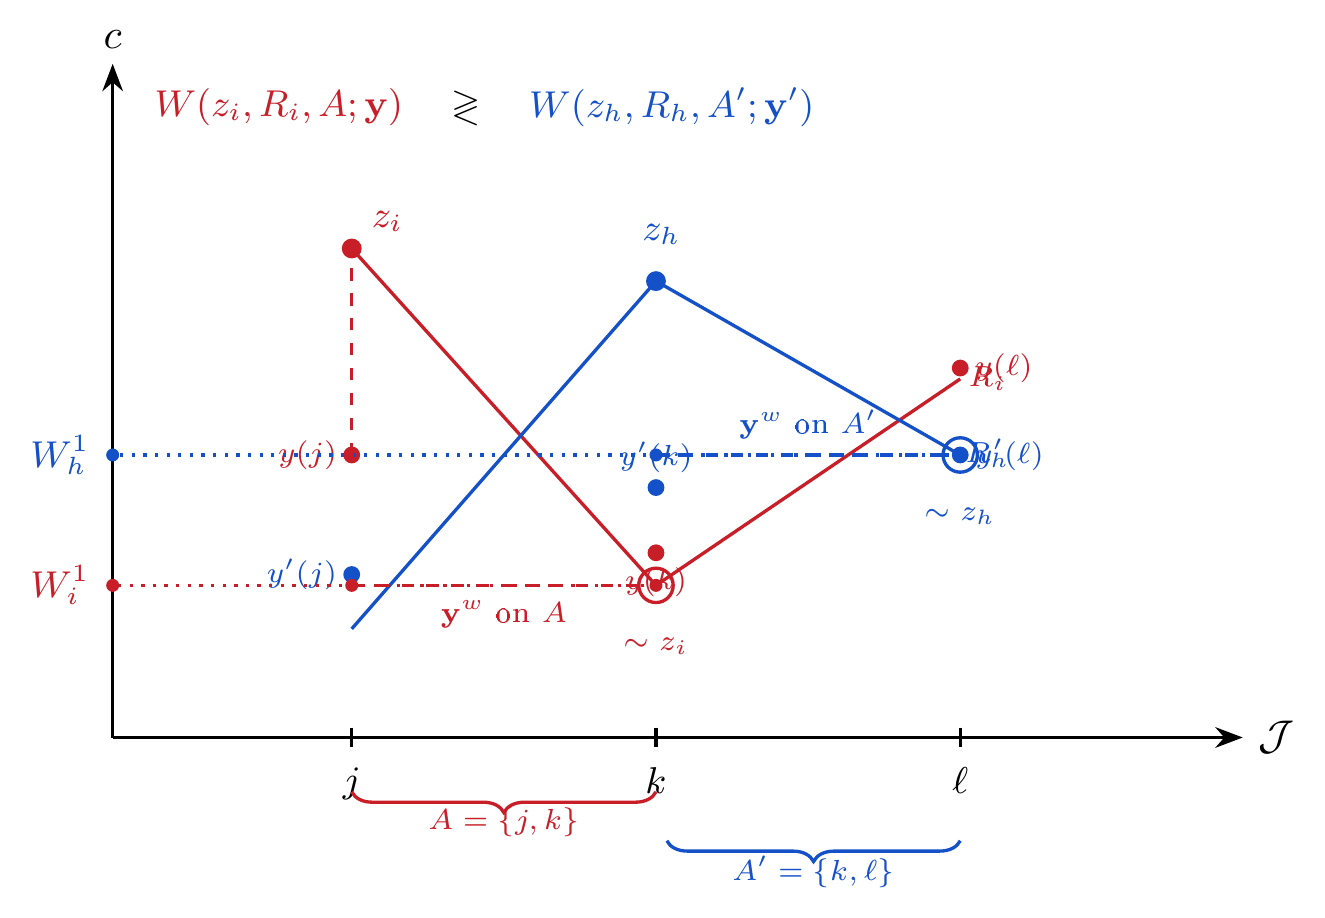
\includegraphics[width=0.95\linewidth,height=\textheight,keepaspectratio,alt={Own-set equal-consumption equivalents. Individuals with preferences R\_i,R\_h and ability sets A=\textbackslash\{j,k\textbackslash\} and A\^{}\{\textbackslash prime\}=\textbackslash\{k,\textbackslash ell\textbackslash\} attain z\_i and z\_h. For each individual, a common consumption level is assigned to every job in their own set; the level at which the preferred reference job becomes indifferent to the attained bundle is the money metric. Adapted from Haydar and Maniquet (2026), work in progress. This is the deterministic construction; the estimated measure is its ex-ante extension, defined in Section 4.}]{figures/v5/theory_w1.png}
\caption{\textbf{Own-set equal-consumption equivalents.} Individuals with preferences \(R_i,R_h\) and ability sets \(A=\{j,k\}\) and \(A^{\prime}=\{k,\ell\}\) attain \(z_i\) and \(z_h\). For each individual, a common consumption level is assigned to every job in their own set; the level at which the preferred reference job becomes indifferent to the attained bundle is the money metric. Adapted from Haydar and Maniquet (2026), work in progress. This is the deterministic construction; the estimated measure is its ex-ante extension, defined in Section 4.}
\end{figure}

We adapt this principle to an estimated distribution of latent jobs. The empirical object is not the deterministic maximum but its ex-ante counterpart: the household's evaluation of the reference prospect, integrated over the jobs it may reach, is set equal to its evaluation of the prospect it actually faces. Section 4 states the stochastic formulation, derives its closed form, and says precisely which properties of the deterministic criterion carry over and which are not claimed.

One comparative static is worth stating plainly at the outset, because it is easy to misread. Holding the attained situation fixed, a person with a larger reference menu may need less uniform consumption to reach the same satisfaction. When actual opportunities change, however, both the attainment and the reference menu change. The net effect on equivalent consumption depends on both. Measuring attainment against one's own opportunities is therefore not a claim that larger menus are intrinsically better, and we make no such claim.

\textbf{The empirical approach.} The behavioural half is a random-utility, random-opportunity model of job choice. A job is a package: an employment state, an occupation, a weekly hours arrangement and an hourly wage. Households rank packages by consumption and leisure, and the packages differ in how available they are. Both the preferences and the household-specific intensity of availability enter one likelihood and are estimated jointly; neither is observed as a complete schedule. Every package is priced through the French tax-benefit system, so a change of hours or occupation moves disposable income through the actual schedule of taxes and transfers rather than a linear approximation. We estimate the model separately on 1,540 single-adult and 2,223 couple households drawn from French EU-SILC, with couples choosing jointly under a shared household budget.

The normative half then yields, for each household, an equivalent flat consumption level. To decompose its inequality we do not linearise. We define four structural equalization operators, one for preferences, one for job access, one for earning opportunities and one for household resources and needs; we recompute every household's welfare level, and the inequality of the resulting distribution, under each of the sixteen coalitions of those operators; and we allocate the interactions among them with the grouped Shapley--Owen--Shorrocks rule. The allocation is exhaustive by construction and the closure is verified numerically rather than imposed.

\textbf{What we find.} Among single-adult households, labour-market opportunities carry 55.92 per cent of the inequality in the money metric, of which job access alone carries 49.16 per cent and earning opportunities 6.76. Preferences carry 9.88 per cent and household resources and needs 34.20. Among couples the composition is different rather than the total: earning opportunities carry 35.72 per cent and resources and needs 51.20, while job access carries only 8.23 and preferences 4.85. Single adults are access-dominated on the labour-market side and couples are earnings- and resource-dominated. We report that contrast as a finding and do not attach a mechanism to it.

Two qualifications belong with the headline. First, the ordering of access against earning opportunities is the robust part: access exceeds earning opportunities for single adults under all six inequality indices we report, and the ordering reverses for couples under all six. The complete ordering of all four components is not robust in that sense, and the sign of the single-adult preference contribution changes outside the Gini. Second, an allocated share is an average of marginal contributions over coalition orders. It is not the reduction that equalizing that group alone would achieve. For single adults the two differ instructively: equalizing preferences alone would \emph{raise} the Gini by 13.0 per cent, while the allocated preference share is a positive 9.88 per cent. Section 5 explains why both statements are correct.

\textbf{Relation to existing work.} Every ingredient here has antecedents, and the contribution is the combination and the empirical answer, not any one step.

Modelling labour supply as choice among latent jobs, with preferences and offer intensities identified jointly from one likelihood, is due to \citet{aaberge1995} and \citet{aaberge1999}, developed by \citet{dagsvikstrom2006} and \citet{dagsvikjia2016}, surveyed by \citet{aaberge2018}, and set out for applied work by \citet{capeau2016}. We inherit that framework, including its distinction between the intensity of an offer and the probability of a choice, and its reliance on excluded opportunity shifters to separate components that choices alone identify only jointly. \citet{capeau2016} also supply two of the identifying restrictions we maintain: the wage-offer distribution is independent of offered hours, and a local unemployment measure shifts availability while being excluded from preferences. Their Belgian application already covers single women, single men and couples, so covering both household types is not itself a contribution.

Combining such a model with a monetary welfare evaluation is also established. \citet{aaberge1995} translate attained utility into an equivalent income against a stated reference household, choice set and tax system, and \citet{aaberge2004} evaluate reforms with joint household choice and restricted hours. \citet{jiathoresen2021} make the case for the job-choice model in exactly this role and report a distribution of compensating variation for a Norwegian reform, and \citet{jacquet2026} compare a standard compensating variation with one computed after replacing preference characteristics by reference values. All four evaluate a \emph{change} between policy regimes. Our object is a cross-sectional distribution of levels under one policy system, and its attribution. A reform gain and a level have different origins and different denominators; a small preference-related reform difference would not imply a small preference share in our decomposition, and our shares do not estimate their reform gains.

The normative half draws on the literature that refuses to resolve interpersonal comparison by assuming common preferences. \citet{fleurbaeymaniquet2006}, \citet{fleurbaeymaniquet2017} and \citet{fleurbaeymaniquet2018} set out how a reference bundle encodes a position on compensation and responsibility; \citet{decosterhaan2015} and \citet{bargain2013} show empirically how much a welfare ordering moves with that choice. Their references fix a wage or an unearned-income intercept and maximize over a deterministic budget set. Ours fixes consumption across the alternatives of an estimated opportunity distribution and integrates. That is a different reference and, as Section 6 records, the ordering is sensitive to it.

The closest decomposition precedents are two. \citet{muehlhan2023} combines a structural labour-supply model with involuntary-unemployment restrictions and a Shapley attribution, decomposing the change in German household \emph{income} inequality into temporal factors and binary restrictions. \citet{creedyherault2011}, in the section that constructs money-metric distributions under alternative policy and population states, decompose a change in inequality and social welfare by averaging over the two orders in which policy and population can be changed; theirs is the closest money-metric welfare-inequality decomposition we know. Both are decompositions of a \emph{change} between two situations, with policy, population or temporal factors as the factors. Ours is a decomposition of a cross-sectional \emph{level} of well-being inequality, with the factors defined as structural operators inside an estimated job-choice model: what a household prefers, which jobs it can reach, what those jobs pay, and what its budget and needs are. The wider behavioural-simulation decomposition tradition, \citet{bargain2012} and \citet{jessen2019}, decomposes income changes in the same spirit.

The allocation rule is inherited outright. \citet{shorrocks1982} states the accounting requirements a decomposition should satisfy; \citet{shorrocks2013} places the Shapley value at the centre of distributional decomposition; \citet{owen1977} supplies the value for games with a priori unions, which is what a grouped allocation requires; \citet{sastretrannoy2002} documents how much the answer can depend on how the exercise is set up; and \citet{audoly2025} give the contemporary practitioner's account of the grouped nonlinear case we use. We claim no new allocation principle. Complete recomputation of every coalition, rather than a linear approximation, likewise has precedents and is better described as methodological discipline than as a contribution.

What is new, to our knowledge, is the conjunction: a random-utility random-opportunity model of job choice, an opportunity-sensitive money-metric welfare level built on the own-set equal-consumption reference, a structural preference/access/earnings/resources game whose operators are defined inside that estimated model, complete recomputation of welfare and inequality under every coalition, and a grouped allocation of the result. The application-specific methodological contribution is the game and its counterfactual operators. The cooperative-game allocation rule is inherited.

\textbf{Roadmap.} Section 2 describes the data and the household budget construction. Section 3 presents the latent-jobs model, its identifying restrictions and its estimation. Section 4 defines the money-metric welfare measure and the structural decomposition. Section 5 reports the behavioural and welfare results for both household types. Section 6 examines sensitivity and states the limitations. Section 7 concludes.

